\documentclass[11pt]{article}
\usepackage[a4paper,margin=2cm]{geometry}
\usepackage{graphicx,booktabs,amsmath,float,caption}
\usepackage[hidelinks]{hyperref}
\setlength{\parskip}{4pt}\setlength{\parindent}{0pt}

\title{\textbf{PRML Lab 9 --- Clustering}}
\author{Aryan Tiwari (B20AI056)\\CSL2050 Pattern Recognition \& Machine Learning, Winter 2022}
\date{}

\begin{document}
\maketitle

\section*{Question 1 --- k-means on the Wine dataset}

\textbf{Pre-processing.} 178 wines, 13 chemical measurements, no missing values or duplicates. The first column (cultivar) is a label;
the clustering does not use it, and it is only consulted afterwards to check the result. The features have very different scales (Proline is
about 750, Hue about 1). k-means uses Euclidean distance, so without scaling Proline alone would decide the clusters. Every feature was
therefore \textbf{standardised} to zero mean and unit variance.

\textbf{a. Dimension reduction and a visual choice of $k$.} PCA to two dimensions keeps 55.4\% of the variance (36.2\% + 19.2\%).
\begin{figure}[H]\centering
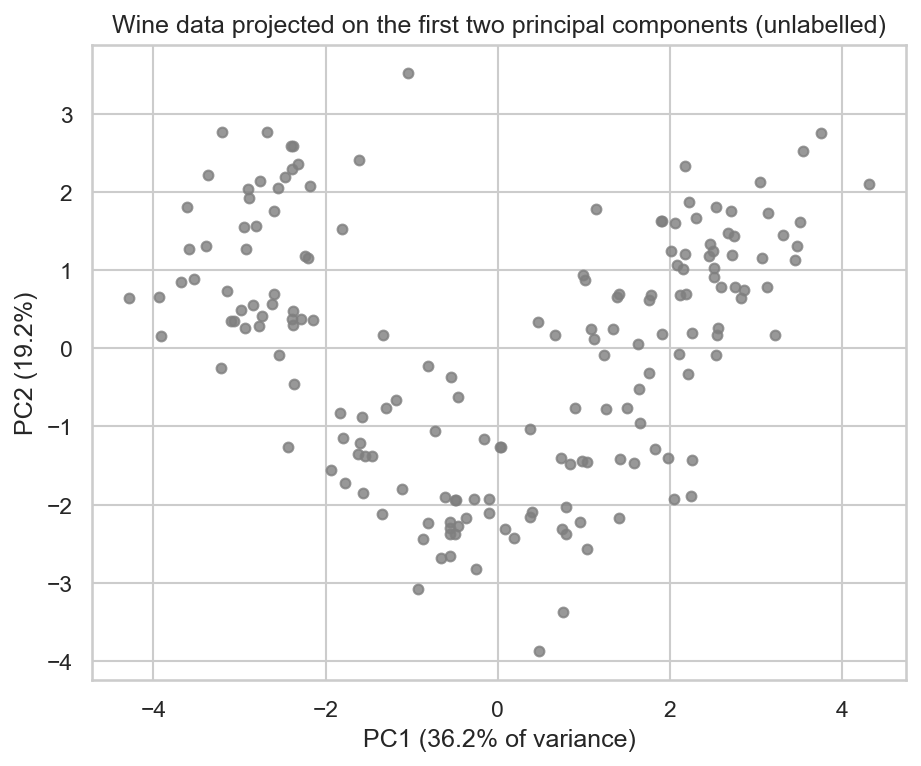
\includegraphics[width=0.5\linewidth]{figures/q1a_pca.png}
\caption{Unlabelled wines in the first two principal components.}
\end{figure}
The points form an arc with \textbf{three dense groups}: one on the left, one at the bottom centre and one on the right, with sparser
regions between them. So I chose \textbf{$k=3$}: $k=2$ would merge two visible groups, and $k\ge4$ would split a compact group.

\textbf{b. k-means with $k=3$.} The clusters have 51, 65 and 62 wines, and their centroids sit in the middle of the three groups.
\begin{figure}[H]\centering
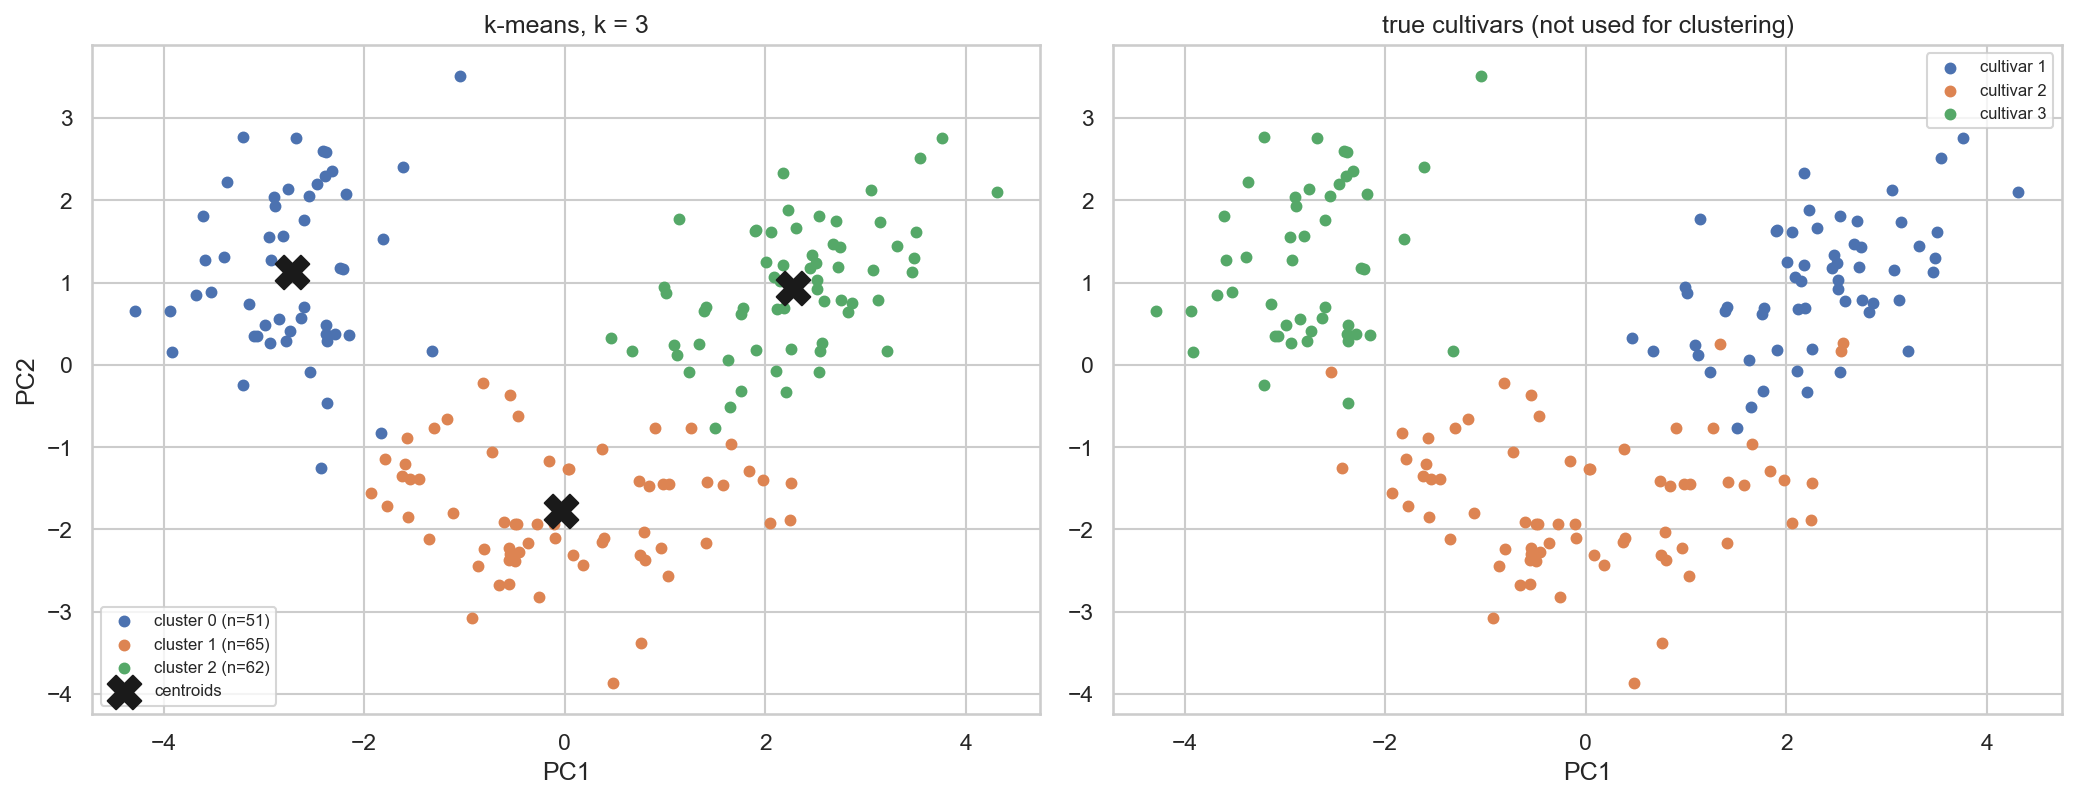
\includegraphics[width=0.9\linewidth]{figures/q1b_kmeans.png}
\caption{k-means clusters with centroids (left) and, for reference only, the true cultivars (right).}
\end{figure}
Compared with the hidden cultivar labels, the clusters are almost exactly the three cultivars: only 6 of 178 wines are in the
``wrong'' cluster (adjusted Rand index \textbf{0.898}). The chemistry really does separate the three grape varieties.

\textbf{c--d. Silhouette and elbow.}
\begin{figure}[H]\centering
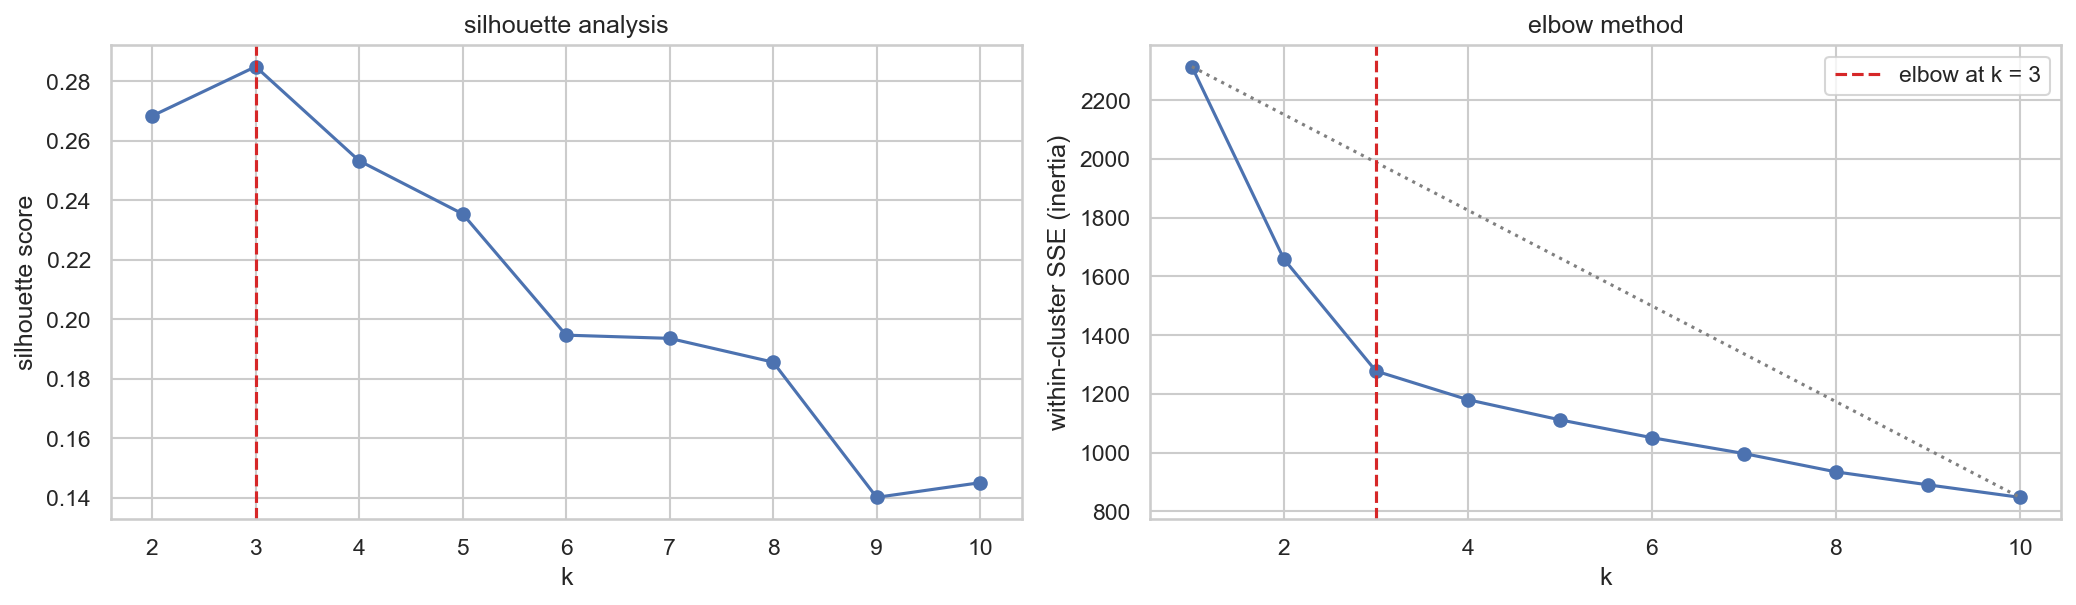
\includegraphics[width=0.9\linewidth]{figures/q1cd_k_selection.png}
\caption{Silhouette score for $k=2..10$ (left) and the elbow curve (right).}
\end{figure}
The silhouette score (how much closer a point is to its own cluster than to the nearest other cluster) is highest at \textbf{$k=3$
(0.285)}, ahead of $k=2$ (0.268) and $k=4$ (0.253), and it keeps falling as $k$ grows. For the elbow method I located the knee objectively, as the point
of the inertia curve farthest from the straight line joining $k=1$ and $k=10$; that is also \textbf{$k=3$}. Up to $k=3$ each extra centre
removes a lot of within-cluster error; after that the gains are small, because the extra centres only cut existing groups. The visual estimate,
the silhouette and the elbow all agree on $k=3$, which is also the true number of cultivars.

\section*{Question 2 --- k-means from scratch on Fashion-MNIST}

The 60{,}000 training images were flattened to 784-dimensional vectors and scaled from 0--255 to [0, 1]. Scaling does not change which centre
is nearest, but it keeps distances and SSE readable and makes the ``input range'' for random initialisation simply $[0,1]^{784}$.

\textbf{a--b. The \texttt{KMeansScratch} class} stores the centres and assignments, takes $k$ and, optionally, the initial centres from
the user, and stops when the largest centre shift falls below $10^{-6}$ (converged) or after \texttt{max\_iter} iterations. Distances use
$\|x-c\|^2=\|x\|^2-2x^\top c+\|c\|^2$, so each iteration is a single matrix product. A cluster that loses all its points keeps its old
centre; no cluster ended up empty in either run below.

\textbf{c--e. Random initialisation} (10 points drawn uniformly from $[0,1]^{784}$). It converged after 41 iterations (5\,s). Points per
cluster: 7660, 8995, 4270, 4307, 8195, 7253, 6137, 6561, 2904, 3718.
\begin{figure}[H]\centering
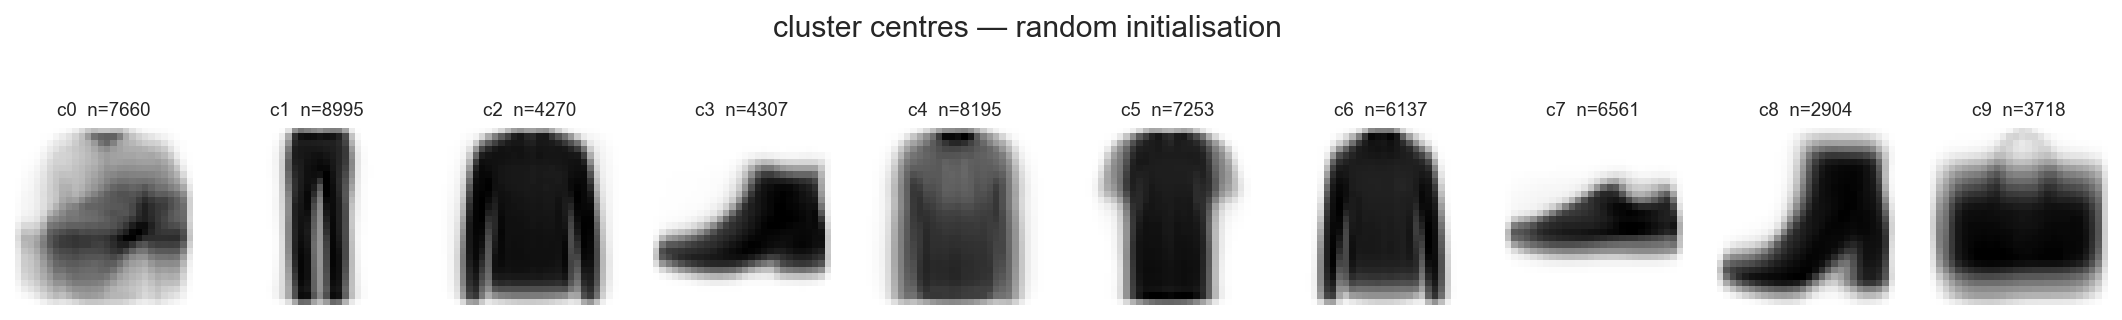
\includegraphics[width=\linewidth]{figures/q2d_centers_random.png}
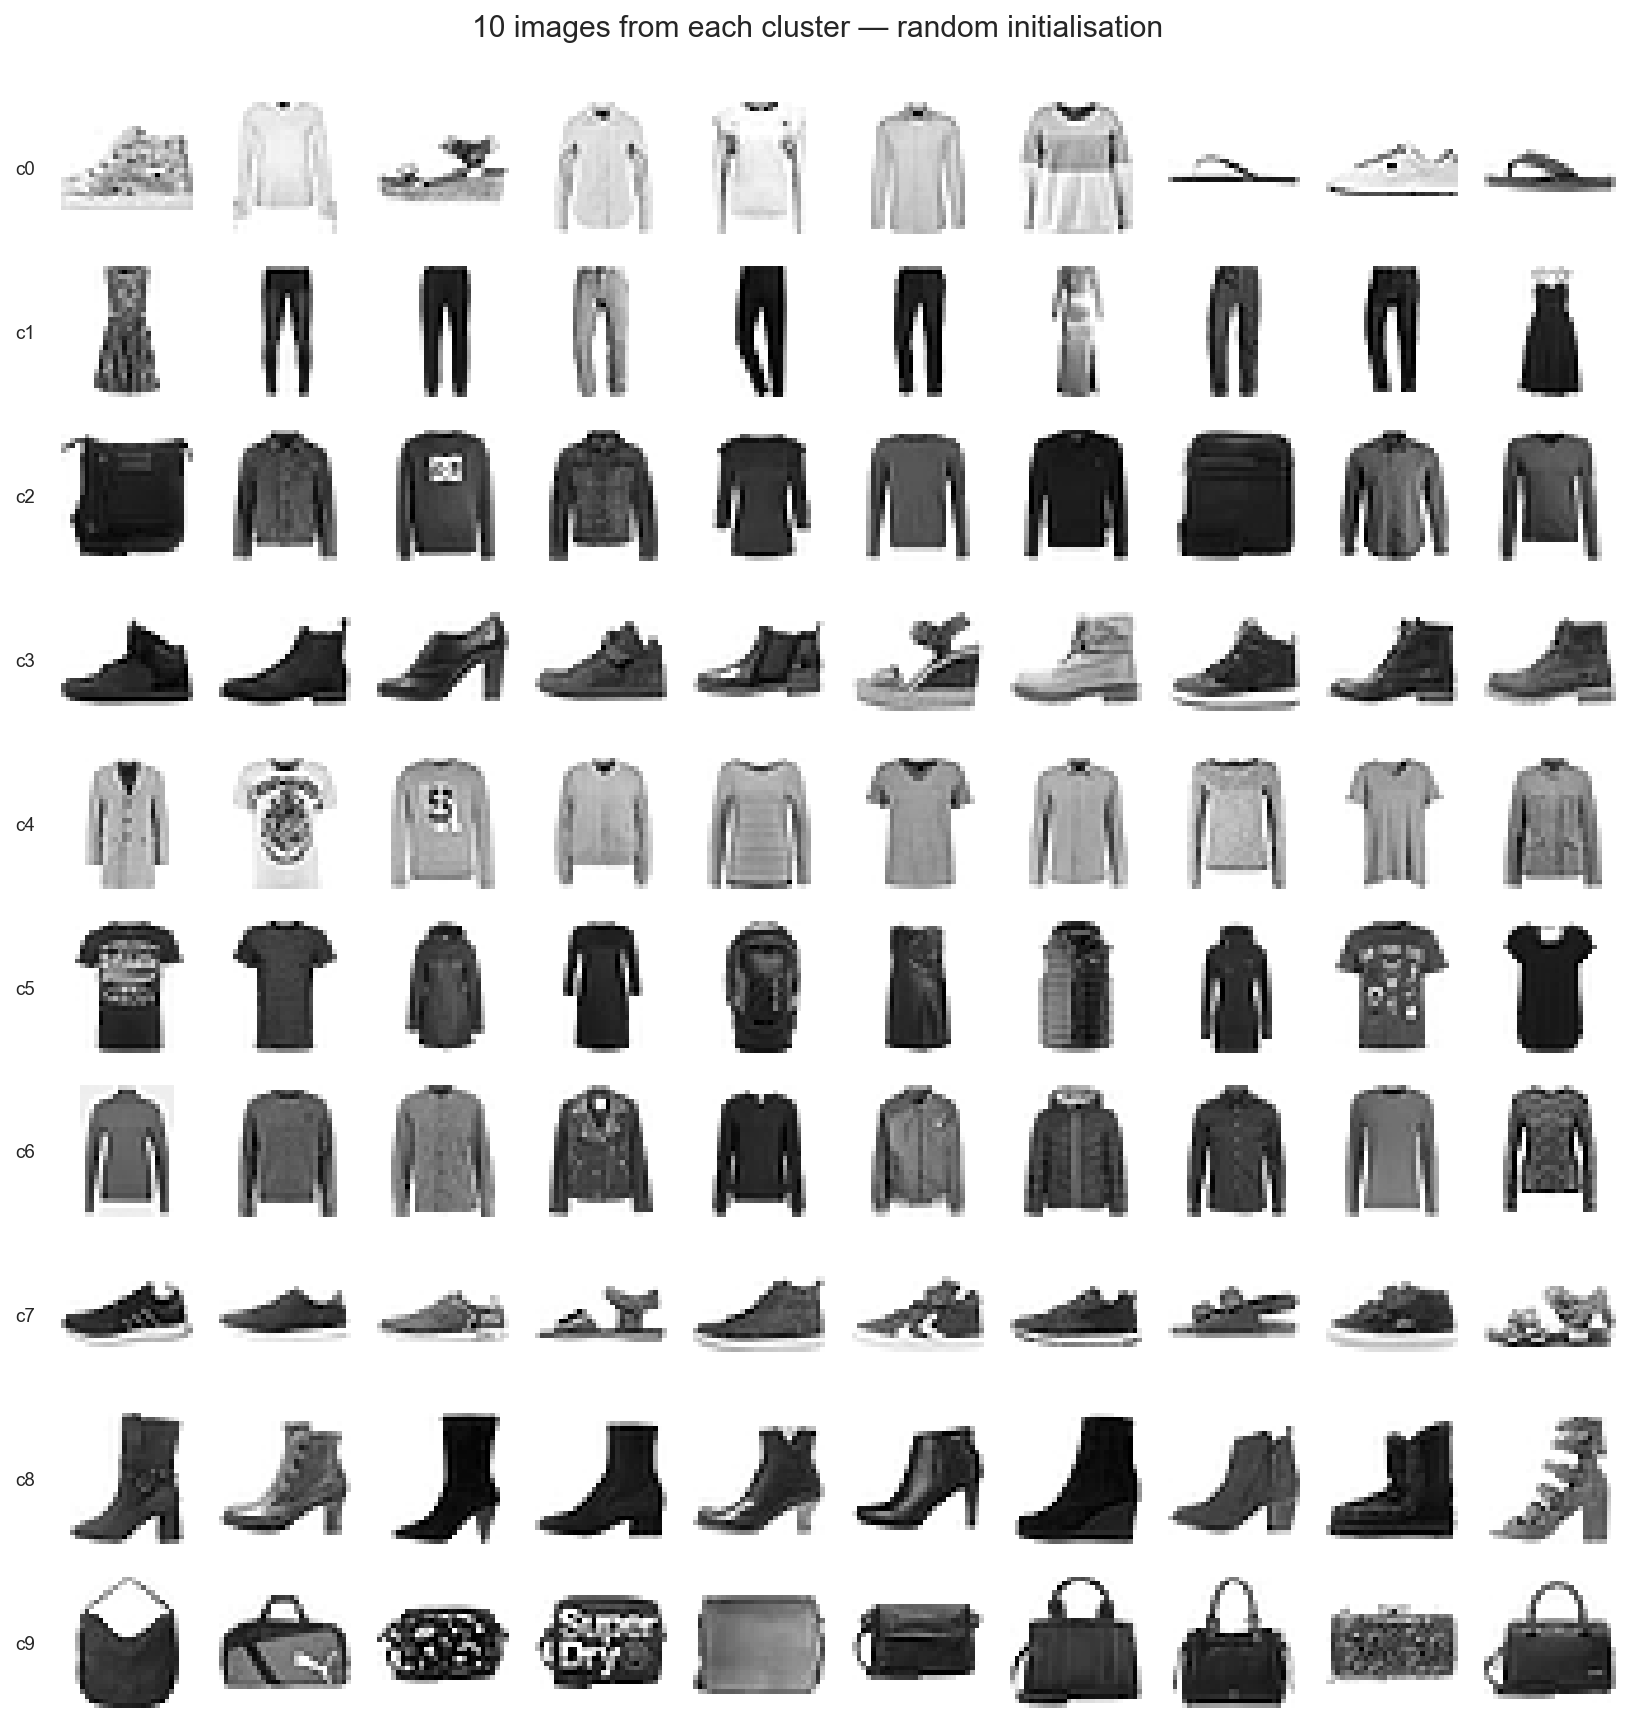
\includegraphics[width=0.62\linewidth]{figures/q2e_members_random.png}
\caption{Cluster centres (top) and 10 random members of each cluster (bottom), random initialisation.}
\end{figure}

\textbf{f--g. Class-based initialisation} (the first training image of each of the 10 classes as the starting centres). It converged after 155
iterations (19\,s). Points per cluster: 6380, 5228, 9534, 5194, 7306, 8010, 2542, 7620, 2356, 5830.
\begin{figure}[H]\centering
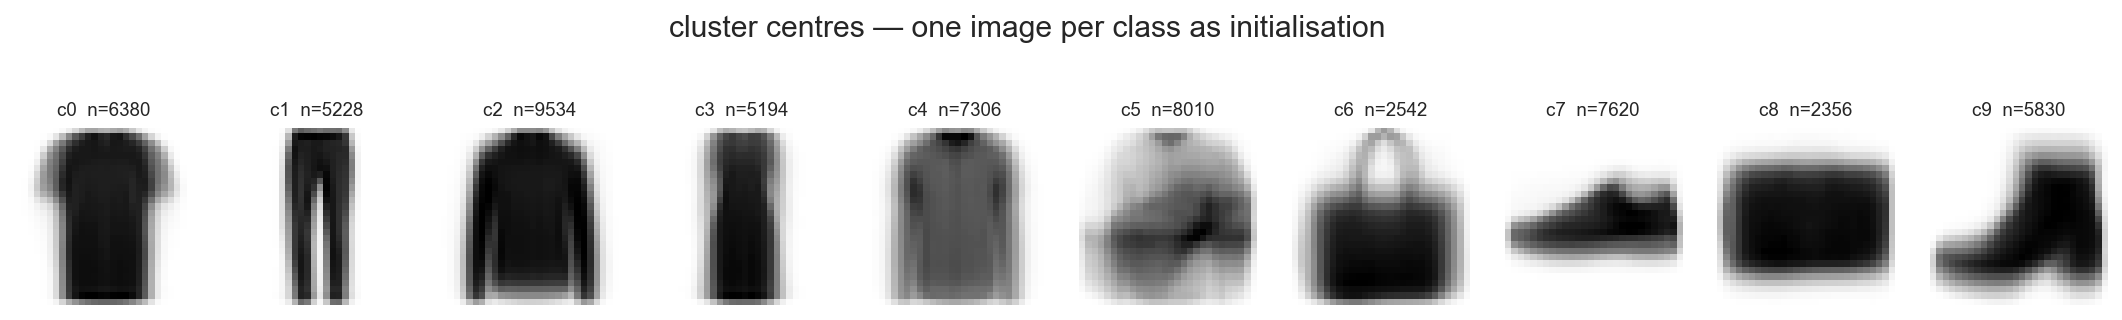
\includegraphics[width=\linewidth]{figures/q2f_centers_class.png}
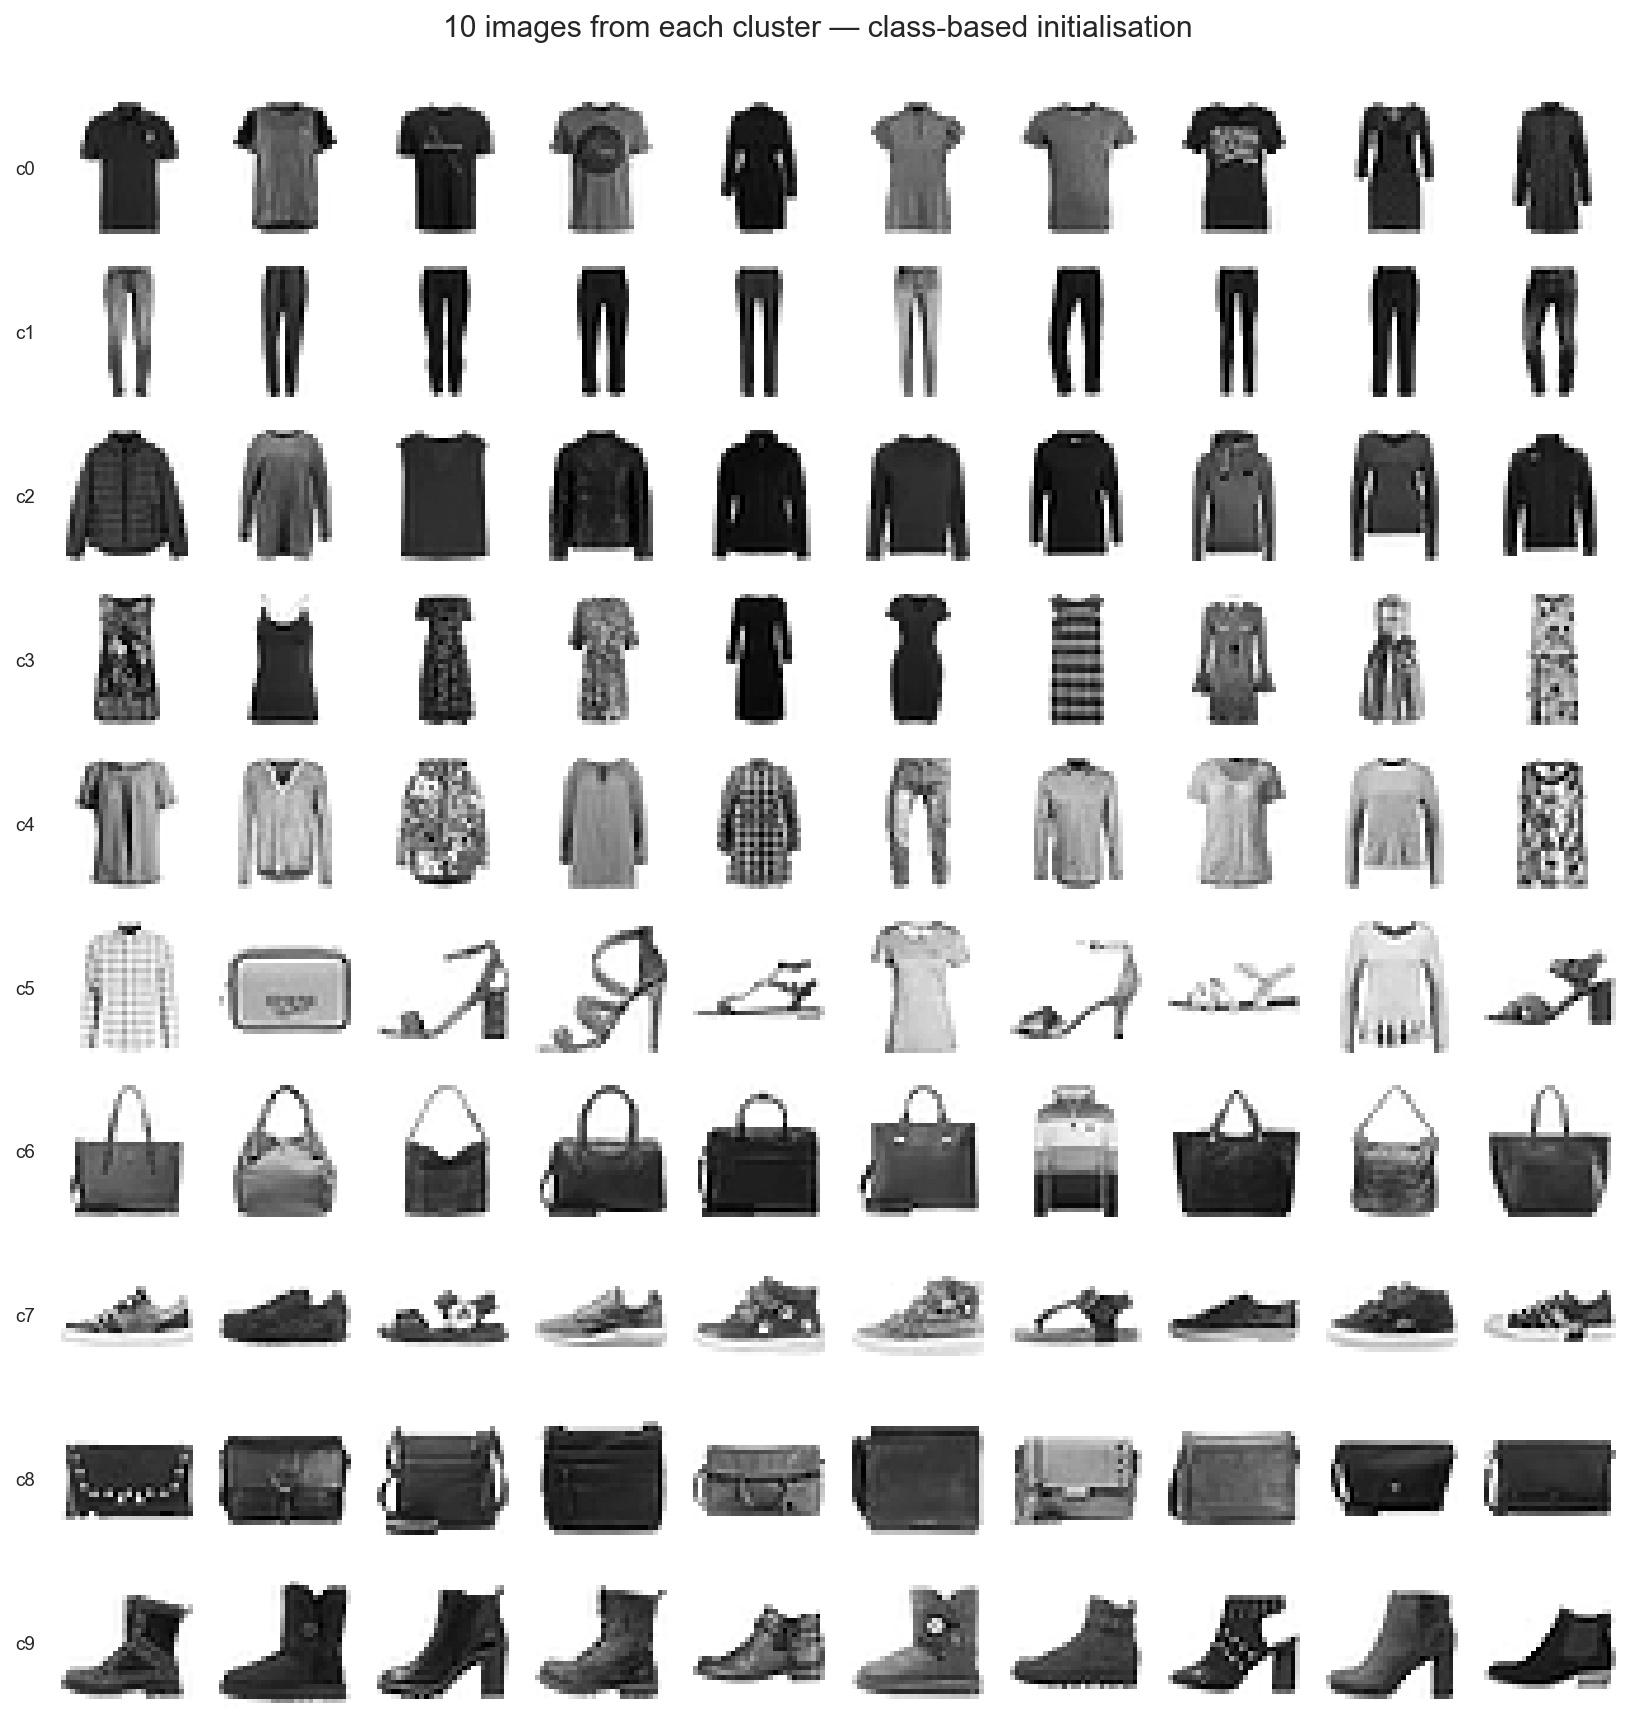
\includegraphics[width=0.62\linewidth]{figures/q2g_members_class.png}
\caption{Cluster centres and members, class-based initialisation.}
\end{figure}

\textbf{h. SSE and comparison.}
\begin{table}[H]\centering
\begin{tabular}{lccccc}\toprule
Initialisation & SSE & Iterations & Non-empty & Purity & ARI vs.\ classes\\\midrule
random (c) & 1{,}923{,}418 & 41 & 10 & 0.556 & 0.342\\
one image per class (f) & \textbf{1{,}919{,}627} & 155 & 10 & \textbf{0.611} & \textbf{0.402}\\\bottomrule
\end{tabular}
\end{table}
\textbf{The class-based initialisation gives the better clustering.} Its SSE is lower, although only by 0.2\%: both runs reach similar local minima of the same objective.
The difference is much clearer in how well the clusters match the real categories: purity rises from 55.6\% to 61.1\% and ARI from 0.34 to 0.40.
Starting each centre in a different class's region steers k-means towards a partition that resembles the classes. Random points in
$[0,1]^{784}$ look like grey noise, far from any garment, so the first assignment step is essentially arbitrary.

Even so, no initialisation makes k-means recover the 10 classes. Two clusters end up as bags, while Pullover, Coat and Shirt share
clusters (see the composition heatmap in the notebook). k-means minimises pixel-wise Euclidean distance, so it groups images by
silhouette and how much ink they have, not by garment type. A pullover, a coat and a long-sleeved shirt have almost the same outline.

\begin{figure}[H]\centering
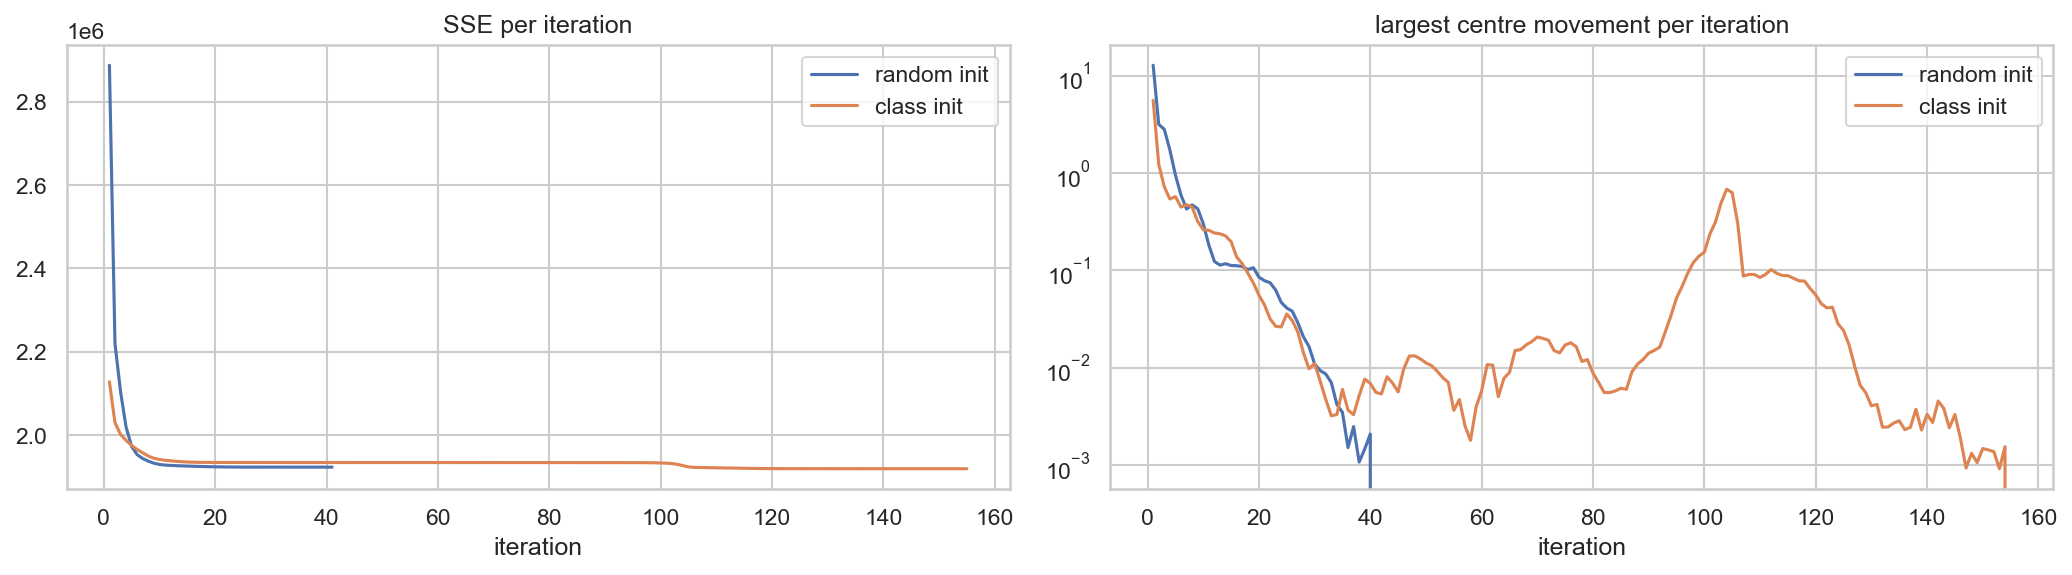
\includegraphics[width=0.8\linewidth]{figures/q2h_convergence.png}
\caption{SSE and largest centre movement per iteration for both runs.}
\end{figure}

\section*{Question 3 --- Hierarchical clustering on the brain MRI dataset (Br35H)}

\textbf{A. Data and normalisation.} 3{,}000 axial brain MRI slices, 1{,}500 with a tumour and 1{,}500 without, in 291 different sizes
(150$\times$167 to 1920$\times$1427). Each image was converted once to 64$\times$64 greyscale, so every image is a vector of 4{,}096 pixel
variables. Every pixel position was then standardised across the dataset so that all variables have the same scale. The tumour label is kept aside for evaluation only.

\begin{figure}[H]\centering
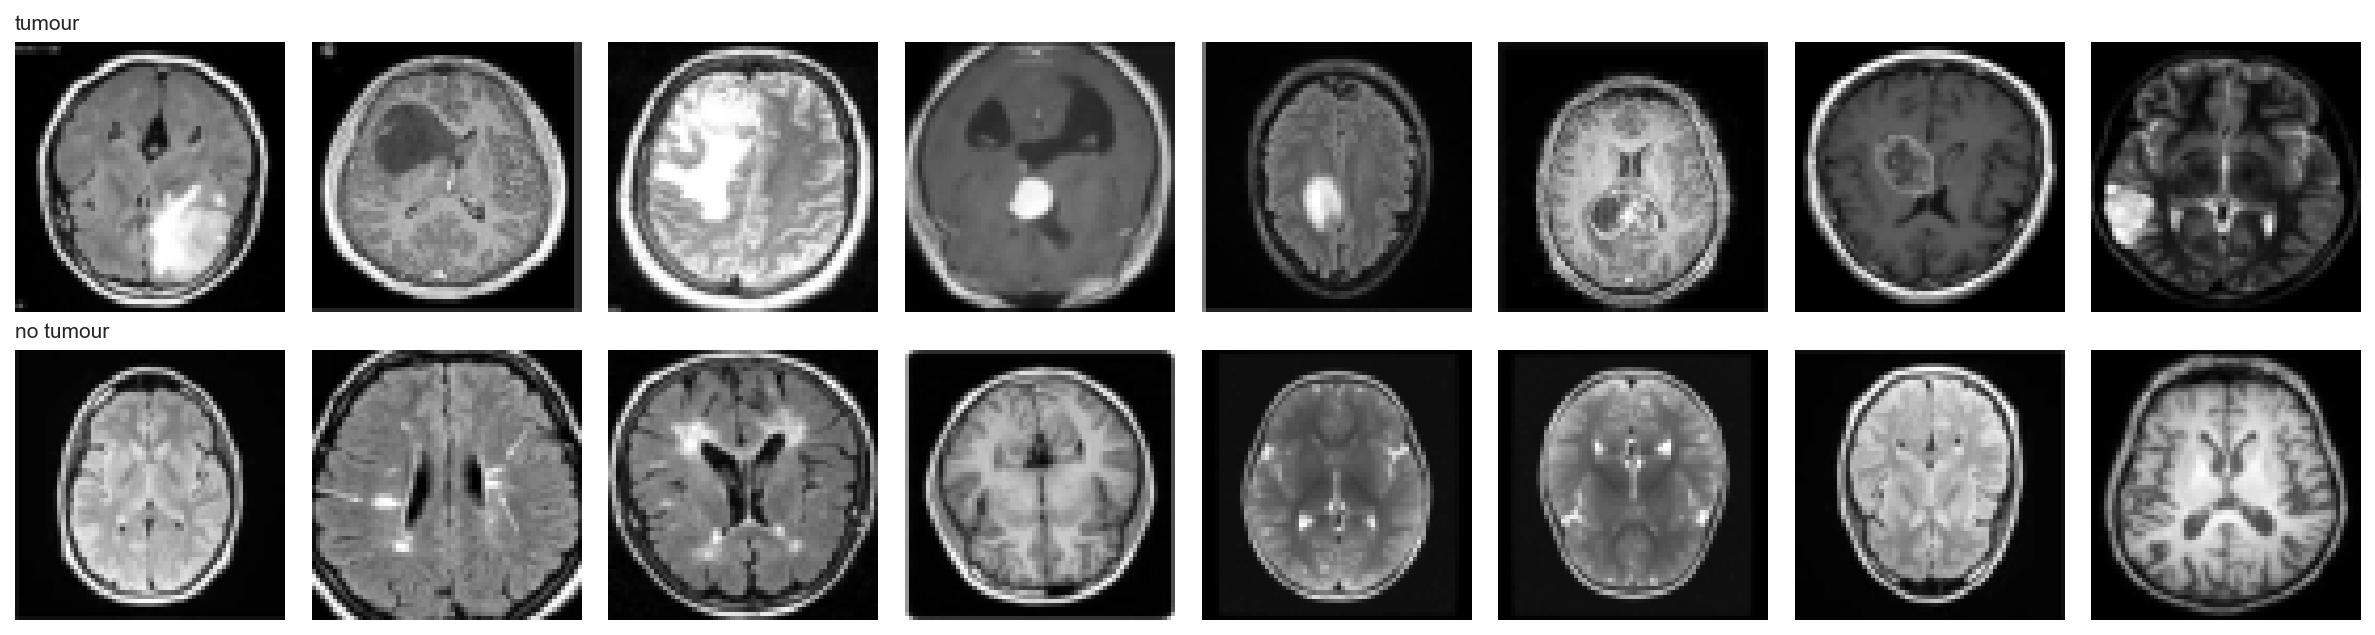
\includegraphics[width=0.85\linewidth]{figures/q3a_samples.png}
\caption{Random samples with (top) and without (bottom) a tumour.}
\end{figure}

\textbf{B--C. Dimension reduction and number of communities.} PCA to 50 components keeps 78.5\% of the variance (PC1 28.0\%, PC2 10.8\%),
and t-SNE on those 50 components gives a 2-D view. The silhouette score over $k=2..8$ is highest at \textbf{$k=2$ (0.265)}, followed by $k=3$ (0.247),
then falls to 0.10--0.14 for $k\ge4$, so the data contains \textbf{two communities}.
\begin{figure}[H]\centering
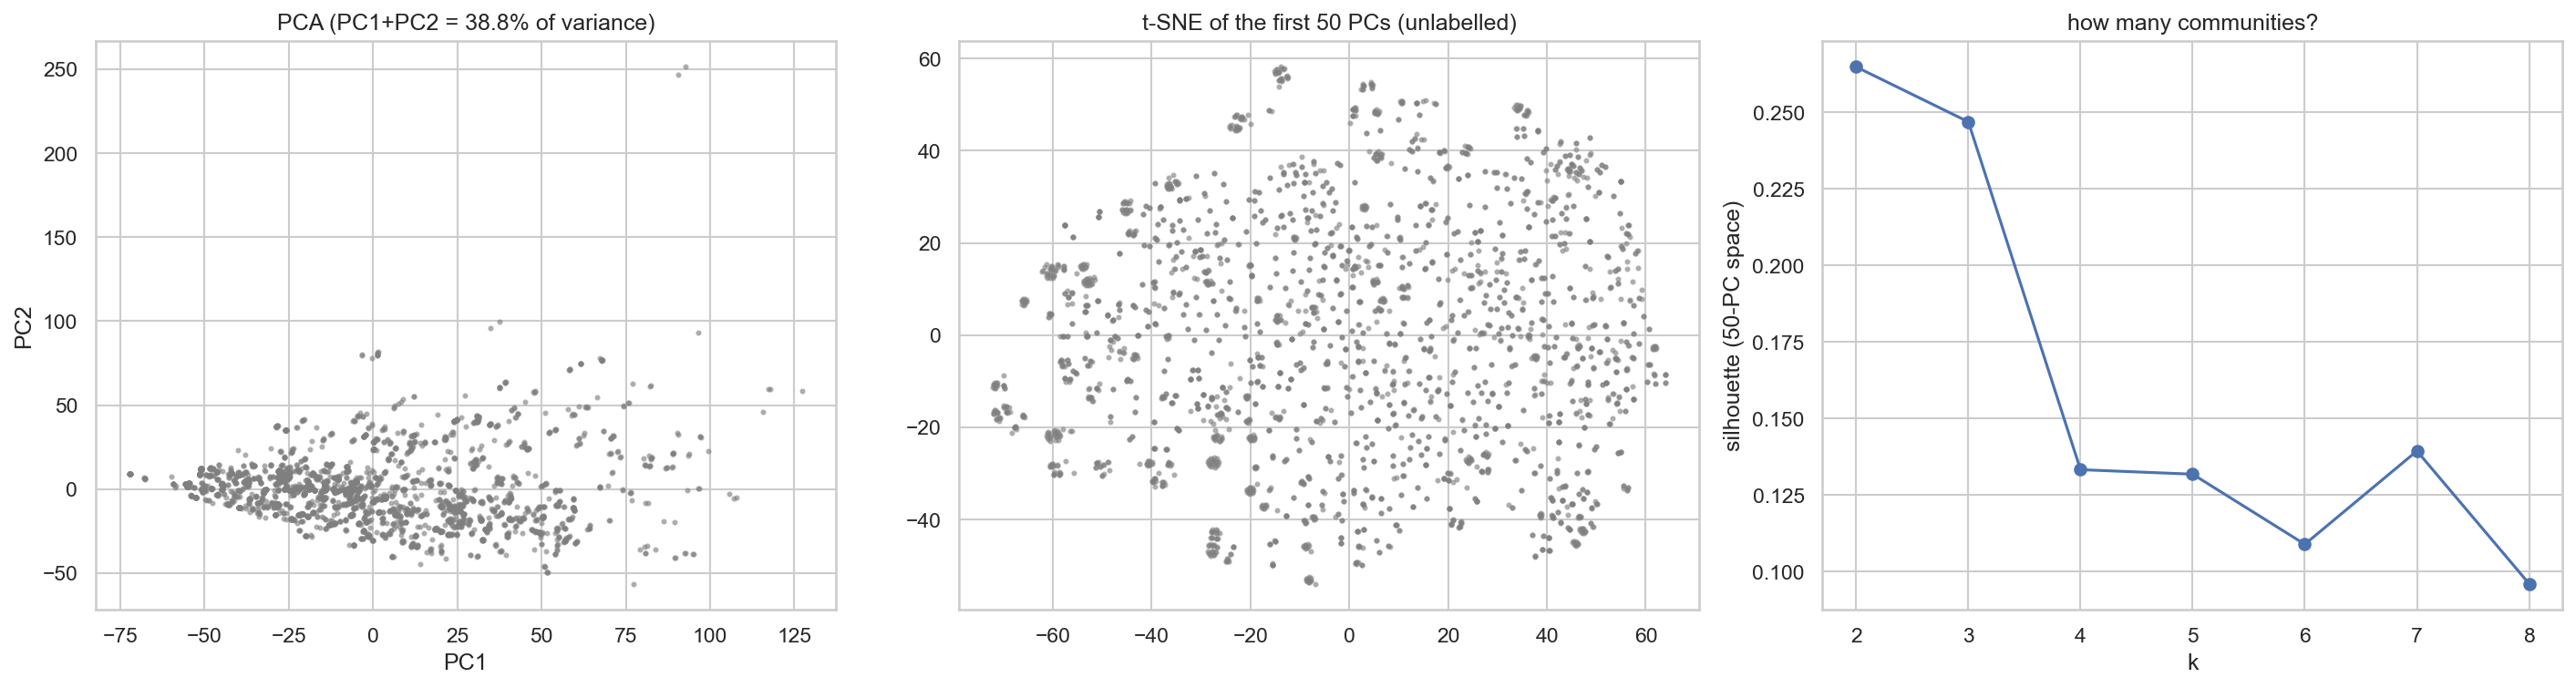
\includegraphics[width=\linewidth]{figures/q3b_reduction.png}
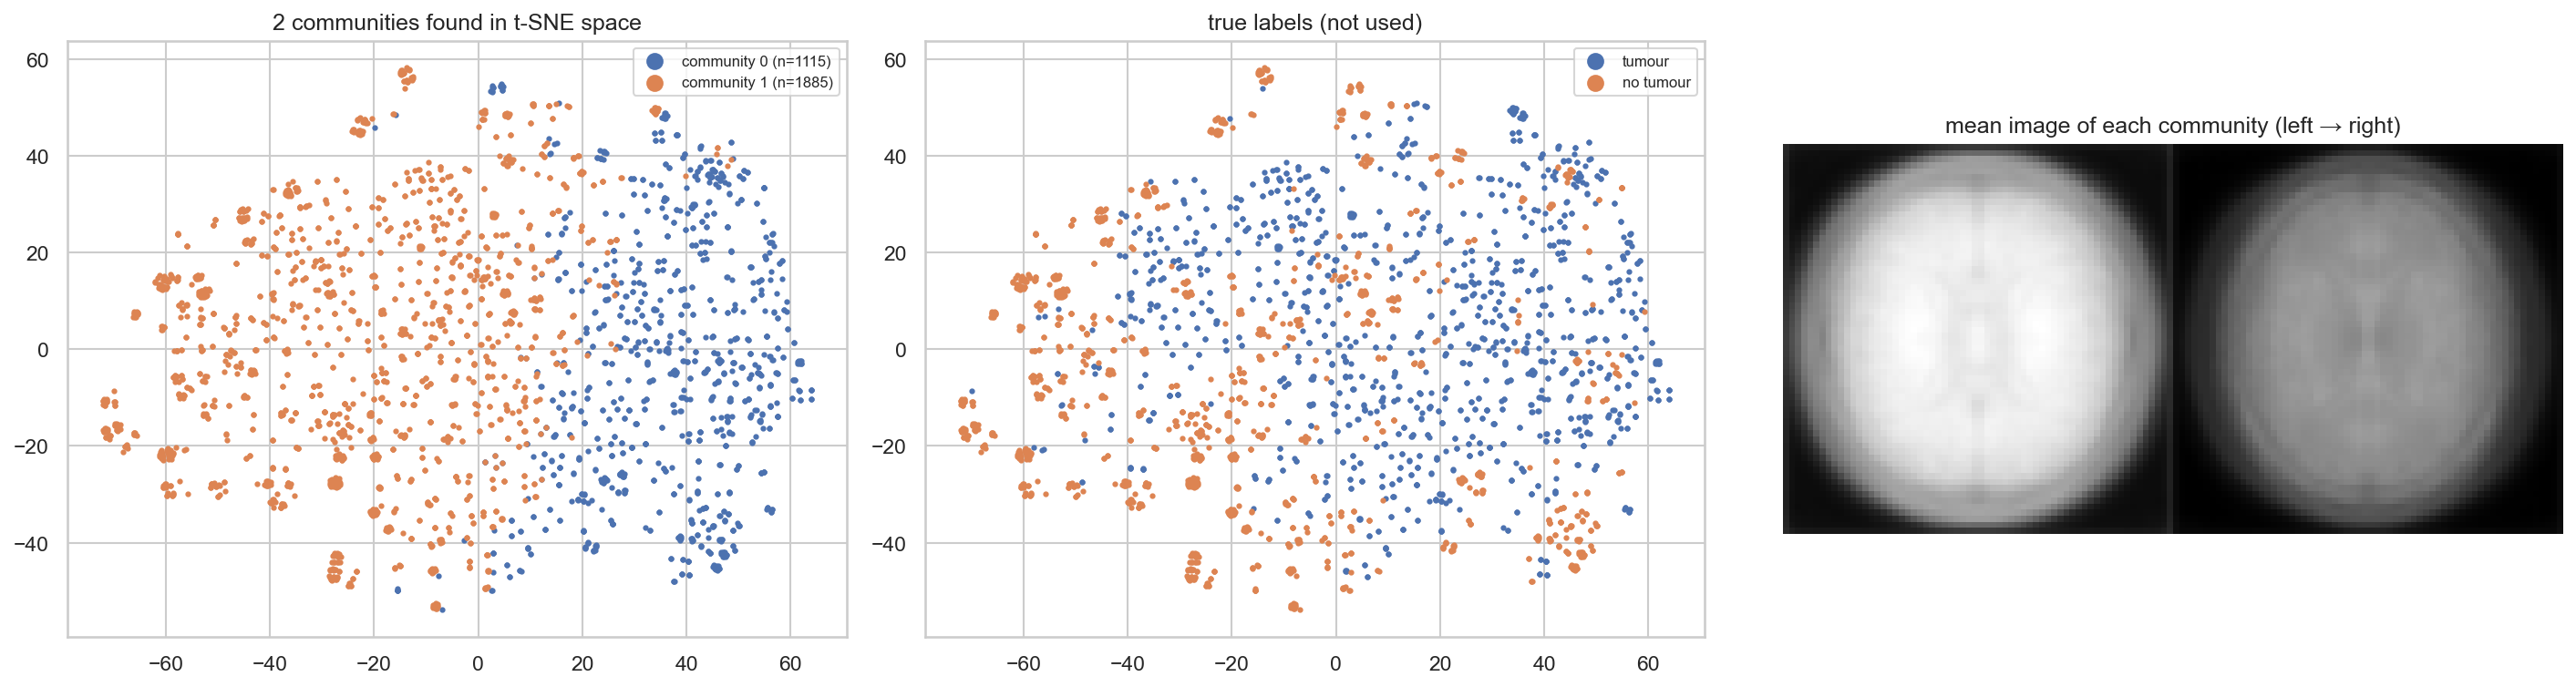
\includegraphics[width=\linewidth]{figures/q3c_communities.png}
\caption{Top: PCA, t-SNE and silhouette by $k$. Bottom: the two communities, the true labels for comparison, and the mean image of each community.}
\end{figure}
The mean images show what the two communities \emph{are}: a \textbf{bright, large-brain} group (1{,}115 images) and a \textbf{darker} group
(1{,}885). The unsupervised structure is driven by overall intensity and head size, which reflect scanner settings and slice position, not by
the tumour. The two only partly overlap: tumour scans are brighter on average (mean pixel 81.7 vs.\ 61.0), so the bright community is 71\% tumour.
A second effect is visible in the t-SNE plot: the healthy scans form many tight clumps, because \textbf{77\% of healthy images have a near-identical twin}
in the dataset, compared with 20\% of tumour images. The ``no'' half of Br35H contains many augmented copies of the same slices.

\textbf{D--E. Agglomerative (Ward) vs.\ k-means} (both with 2 clusters, on the 50 PCs):
\begin{table}[H]\centering
\begin{tabular}{lccccc}\toprule
Method & Cluster sizes & Silhouette & Purity vs.\ tumour & ARI vs.\ tumour & Time (s)\\\midrule
Agglomerative (Ward) & 936 / 2064 & 0.251 & 0.631 & 0.068 & 0.10\\
k-means & 1115 / 1885 & \textbf{0.265} & \textbf{0.659} & \textbf{0.101} & 0.06\\\bottomrule
\end{tabular}
\end{table}
\begin{figure}[H]\centering
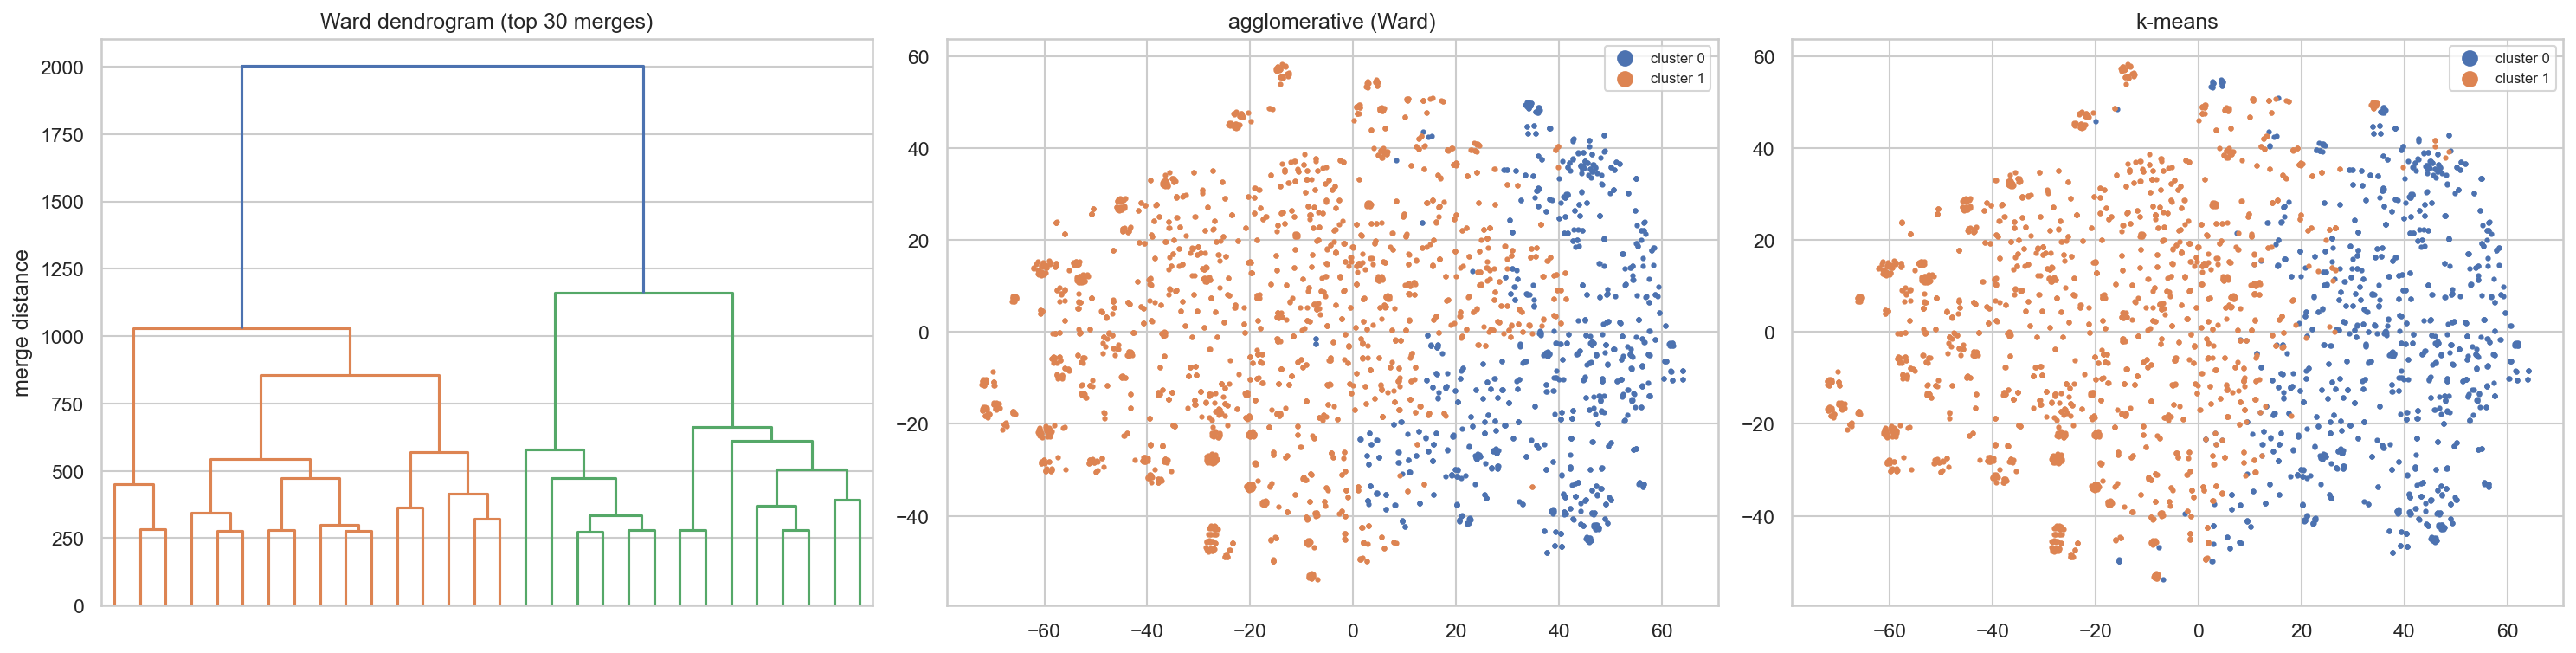
\includegraphics[width=\linewidth]{figures/q3de_compare.png}
\caption{Ward dendrogram (top 30 merges) and the two clusterings in t-SNE space.}
\end{figure}

The two methods find broadly the same split: they agree with each other at ARI 0.63, far more than either agrees with the tumour label. k-means
scores slightly better on every measure. Ward linkage also minimises within-cluster variance, but it does so greedily: once two groups merge
they can never be separated again. An early merge of borderline images therefore stays in the final partition, and Ward's bright cluster ends up smaller (936 against 1115).
k-means keeps reassigning points until it converges, so it finds a better local optimum of the same variance objective. The dendrogram shows one very large final
merge, which supports a 2-community structure, but neither method separates tumour from healthy brains (ARI $\le$ 0.10). Without labels, the
largest source of variation in raw pixels is brightness and anatomy, and the tumour, a small local region, contributes little to the
distance between whole images. Separating the classes would need features that focus on the lesion, or a supervised model.

\end{document}
